\chapter{Investor and Executive Doug Williams: Focus, Scale, and Character}

These notes follow the School of Hard Knocks interview with Doug Williams, former chief operating officer of HMS Holdings and now an investor and board member. There is no blackboard mathematics in the source frames, so the mathematical structure here is deliberately modest: we preserve the numbers, ratios, valuation language, and operating sequences that the transcript actually gives. The spine of the chapter is commercial rather than physical: how capital is allocated, how small firms earn credibility, how sales become diagnosis, how scale is planned in advance, and why trust matters when plans fail.

\section{Investment Filters Before Investment Stories}

The interview begins with a credential and then immediately turns to the practical question: what does Williams look for when investing? The credential matters. HMS Holdings, he says, was a healthcare company sold for about \(\$3.5\) billion. That is not offered as a formula; it is offered as the standing from which the rest of the advice is spoken.

Williams then describes the investing vehicle and the stage of company it targets:
\begin{equation}
C_{\mathrm{fund}} \approx \$50\,\mathrm{M}.
\end{equation}
The fund is venture-oriented and early-stage. The checks are not tiny angel checks and not large buyout checks:
\begin{equation}
\$0.5\,\mathrm{M} \lesssim I_{\mathrm{check}} \lesssim \$3\,\mathrm{M}.
\end{equation}
The companies are often still small in revenue terms:
\begin{equation}
R_{\mathrm{startup}} \lesssim \$2\,\mathrm{M}.
\end{equation}

The filter is not only numerical. Williams names interesting ideas, thoughtful management teams, and large target markets. The numbers set the stage; the people and the market decide whether the stage is worth entering.

\begin{table}
\centering
\begin{tabular}{ll}
Object & Transcript-grounded value or criterion \\
Fund capacity & about \(\$50\,\mathrm{M}\) \\
Typical check & about \(\$0.5\,\mathrm{M}\) to \(\$3\,\mathrm{M}\) \\
Company revenue & probably below \(\$2\,\mathrm{M}\) \\
Target market & large enough to matter \\
Management & thoughtful, coachable, focused \\
Investor role & organize, hire talent, maintain focus \\
\end{tabular}
\end{table}

The movement is from capital to attention. Williams does not present money as the main constraint. The young company has too many possible actions, too few people, and not enough clarity about what matters.

\section{From Smart Founder to Sellable Message}

The first concrete coaching example is a founder who is smart, knows the market, and understands the product. That is still not enough. The message may fail to ``ring the bell.'' A technically strong company can still lose because the buyer cannot see the problem sharply enough.

Williams's rule is blunt: sell through fear, not foresight. The claim is not that one should manipulate customers. His explanation is narrower. Executives are not primarily afraid of missing upside; they are afraid of failure. A useful sales message identifies the failure that the customer already has reason to avoid.

\subsection{Question \& Answer}

\paragraph{Question.} Why would a large customer listen to a very small company?

\paragraph{Answer.} Because the small company can be attached to a failure the customer already cares about, and because credibility can be transferred through trust. Williams gives the asymmetry in scale as part of the problem:
\begin{equation}
S_{\mathrm{seller}} \approx \$2\,\mathrm{M},
\qquad
S_{\mathrm{buyer}} \approx \$50\,\mathrm{B}.
\end{equation}
A cautious scale comparison is
\begin{equation}
\frac{S_{\mathrm{buyer}}}{S_{\mathrm{seller}}}
\approx
\frac{50\,\mathrm{B}}{2\,\mathrm{M}}
=
25{,}000.
\end{equation}
That ratio is not presented in the interview as a formal calculation, but it makes the problem visible. A small company selling into a massive buyer faces a credibility gap. Williams's mechanism is to lend credibility from long market experience: if the buyer trusts him, it may become easier for the buyer to trust the company he introduces.

The message then has three tests. Is it on track? Does it matter to the people being sold to? Does it explain why the buyer cannot simply buy from someone else?

\section{Sales as Diagnosis, Not Demonstration}

The next question asks how someone can crush sales. Williams answers by reversing the usual performance instinct. No one likes being sold to, he says, but everybody likes to buy. So the salesperson should not begin with the demo. The salesperson should begin with the customer's need.

Let \(P_{\mathrm{client}}\) denote the client's pain point or failure risk. The sales sequence Williams describes can be written as a simple diagnostic chain:
\begin{equation}
\mathrm{Homework}
\longrightarrow
P_{\mathrm{client}}
\longrightarrow
\mathrm{Questions}
\longrightarrow
\mathrm{True\ Need}
\longrightarrow
\mathrm{Solution}.
\end{equation}
The important step is that the product does not enter first. In Williams's version, the product has to wait until the need is understood.

\begin{figure}
\centering
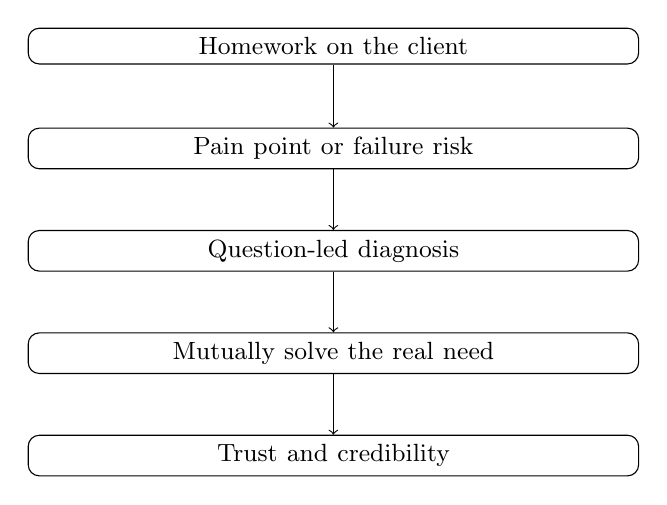
\begin{tikzpicture}[x=1cm,y=1cm]
\node[draw, rounded corners, text width=.62\linewidth, align=center] (a) at (0,0) {\small Homework on the client};
\node[draw, rounded corners, text width=.62\linewidth, align=center] (b) at (0,-1.3) {\small Pain point or failure risk};
\node[draw, rounded corners, text width=.62\linewidth, align=center] (c) at (0,-2.6) {\small Question-led diagnosis};
\node[draw, rounded corners, text width=.62\linewidth, align=center] (d) at (0,-3.9) {\small Mutually solve the real need};
\node[draw, rounded corners, text width=.62\linewidth, align=center] (e) at (0,-5.2) {\small Trust and credibility};
\draw[->] (a) -- (b);
\draw[->] (b) -- (c);
\draw[->] (c) -- (d);
\draw[->] (d) -- (e);
\end{tikzpicture}
\end{figure}

The contrast is with demo-first selling: showing everything and waiting for something to catch. Williams treats that as randomness disguised as energy. The disciplined version slows down, studies the client, and solves a specific problem.

\section{The Folding-Paper Theory of Scale}

The interviewer next asks about scaling from six figures to seven, eight, and beyond. Williams first mentions the valuation language used when companies are sold:
\begin{equation}
EV \approx m_R R
\end{equation}
or
\begin{equation}
EV \approx m_E \,\mathrm{EBITDA}.
\end{equation}
Here \(EV\) denotes enterprise value, \(R\) denotes revenue, \(m_R\) is a revenue multiple, and \(m_E\) is an EBITDA multiple. These are standard notational reconstructions of his phrase ``multiple of revenue or EBITDA.'' The interview does not give the actual transaction multiple for HMS, so we should not invent it.

But Williams does not stay on valuation. He pivots to operating design. To scale, he says, the company must get the basics right: value proposition, total addressable market, customer, and key message. Then comes the visual metaphor: a folding piece of paper.

\subsection{Question \& Answer}

\paragraph{Question.} How does a business scale without merely doing more and more?

\paragraph{Answer.} By designing the next scale state before arriving there. Let \(S_0\) be the current scale of the business. The growth path Williams describes is naturally represented by repeated doubling:
\begin{equation}
S_0 \longrightarrow 2S_0 \longrightarrow 4S_0 \longrightarrow 8S_0.
\end{equation}
At each stage \(S_k\), the company needs a corresponding operating design \(D_k\):
\begin{equation}
D_k =
\{\mathrm{organization},\ \mathrm{metrics},\ \mathrm{alignment},\ \mathrm{relationships},\ \mathrm{channels}\}.
\end{equation}
The point is not the symbol. The point is that \(D_2\) should not be improvised only after the company reaches \(4S_0\). The design is prepared in advance.

\begin{figure}
\centering
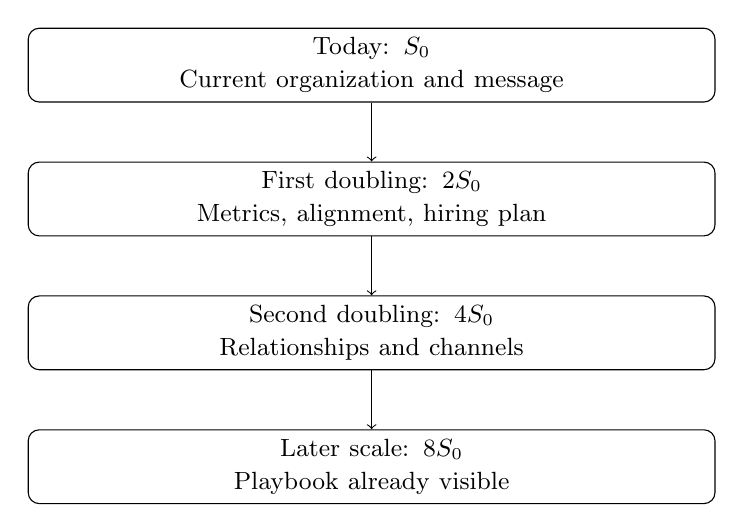
\begin{tikzpicture}[x=1cm,y=1cm]
\node[draw, rounded corners, text width=.7\linewidth, align=center] (s0) at (0,0) {\small Today: \(S_0\)\\\small Current organization and message};
\node[draw, rounded corners, text width=.7\linewidth, align=center] (s1) at (0,-1.7) {\small First doubling: \(2S_0\)\\\small Metrics, alignment, hiring plan};
\node[draw, rounded corners, text width=.7\linewidth, align=center] (s2) at (0,-3.4) {\small Second doubling: \(4S_0\)\\\small Relationships and channels};
\node[draw, rounded corners, text width=.7\linewidth, align=center] (s3) at (0,-5.1) {\small Later scale: \(8S_0\)\\\small Playbook already visible};
\draw[->] (s0) -- (s1);
\draw[->] (s1) -- (s2);
\draw[->] (s2) -- (s3);
\end{tikzpicture}
\end{figure}

\paragraph{Worked example.} Suppose a company is at \(S_0\), and for concreteness we let \(S_0\) stand for current annual revenue. If the present revenue is \(\$1\,\mathrm{M}\), then the doubling path is
\begin{align}
S_0 &= \$1\,\mathrm{M},\\
2S_0 &= \$2\,\mathrm{M},\\
4S_0 &= \$4\,\mathrm{M},\\
8S_0 &= \$8\,\mathrm{M}.
\end{align}
Williams's operating claim is that each of these stages should have a design attached:
\begin{align}
S_0 &\mapsto D_0,\\
2S_0 &\mapsto D_1,\\
4S_0 &\mapsto D_2,\\
8S_0 &\mapsto D_3.
\end{align}
The bad update rule is
\begin{equation}
D_{k+1}=\hbox{whatever we invent after the crisis arrives}.
\end{equation}
The disciplined update rule is
\begin{equation}
D_{k+1}=\hbox{the next design prepared while operating at }D_k.
\end{equation}
This is what removes wasted time and space from scaling. More effort is not the same as prepared structure.

\section{Career Capital: Skills, Mentors, and the Walk}

The interview then turns to Williams's book, \emph{Shift: A Playbook for Positive Change}. The original working title, he says, was something like \emph{Enjoy the Walk} or \emph{Enjoy the Journey}. The shift in the conversation is important. After talking about firms as systems, he turns to careers as compounding paths.

At age sixty-three, Williams says he is still looking ahead, but when he looks back, the things that mattered were the skills learned and the people met. The job title and the company name were not the deepest asset. Mentors, colleagues, and the practice of helping others improve became the durable residue.

We can write this as a simple accounting identity for career capital, not as a financial formula but as a disciplined mnemonic:
\begin{equation}
K_{\mathrm{career}}
=
K_{\mathrm{skills}}
+
K_{\mathrm{relationships}}
+
K_{\mathrm{reputation}}.
\end{equation}
The transcript supports the ingredients, not the equation. The point is to keep separate what the interview treats separately: skill, people, and care for others' progress.

\section{Work, Family, and Sharpening the Axe}

The next question asks whether people can have work-life balance and still be successful. Williams calls it a tough question, then answers with boundaries rather than slogans. He had about
\begin{equation}
M_{\mathrm{American}} \approx 5.5\,\mathrm{M\ miles}
\end{equation}
on American Airlines, so his career involved heavy travel. His rule was that when he was away from home, he worked; when he got home, he was home.

He describes not taking calls all day Saturday and sometimes spending one to one and a half hours on Sunday night preparing for the next week:
\begin{equation}
T_{\mathrm{Sunday\ prep}} \approx 1\hbox{ to }1.5\ \mathrm{hours}.
\end{equation}
This is not a universal calendar prescription. It is an example of a boundary that makes presence possible.

\subsection{Question \& Answer}

\paragraph{Question.} Can work-life balance survive serious ambition?

\paragraph{Answer.} In Williams's account, yes, but only if balance is made operational. It is not a feeling added after the work is done. It is a rule about where attention goes. Work while away; be home when home. The alternative he warns against is the late-career professional who has money but not relationships, friends, or family ties.

The mental-health question continues the same line. Williams says one needs more than one focus in life. His own rhythm starts early:
\begin{equation}
t_{\mathrm{wake}} \approx 4{:}30,
\qquad
t_{\mathrm{gym}} \approx 5{:}00.
\end{equation}
He works out generally seven days a week, sometimes twice in a day. He also names golf, sailing, hiking, and road biking as ways to leave the office mentally.

The metaphor is Abraham Lincoln's axe: if one has four hours to chop down a tree, spend the first three sharpening the axe. Williams uses the story to make a performance point. Renewal is not outside the work. It prepares the person who does the work.

\section{Risk, Trust, and Character Under Stress}

The interview returns to biography before it returns to risk. Williams studied computer science, began as a programmer, and worked in the field with devices, protocols, companies, and people. That path led into Arthur Andersen, healthcare technology, healthcare IBM consulting, and ultimately HMS Holdings.

The financial-decision question begins lightly: he jokes that his worst decision was not buying enough Bitcoin or Tesla. Then he becomes more precise. He has lost money on an investment, but when he looked back at the data and the people he was betting on, he still thought it was a good bet. That distinction matters. A bad outcome is not automatically a bad decision.

Williams then gives the risk rule:
\begin{equation}
\hbox{If every investment succeeds, the risk meter may be too low.}
\end{equation}
This is qualitative, not a formal portfolio theorem. It says that a portfolio with no failures may be avoiding the kind of uncertainty required for venture returns.

\subsection{Question \& Answer}

\paragraph{Question.} What does due diligence miss if it stays inside the pitch deck?

\paragraph{Answer.} It misses character under stress. Williams says to trust your gut and get to know people before investing with them, not only through a demo or PowerPoint presentation. Meet them, talk to them, get offline, understand what people are made of. The reason is simple: no business plan goes off flawlessly.

The diligence chain can be represented narrowly:
\begin{equation}
\mathrm{Pitch}
\longrightarrow
\mathrm{Offline\ relationship}
\longrightarrow
\mathrm{Character}
\longrightarrow
\mathrm{Alignment}.
\end{equation}

\begin{figure}
\centering
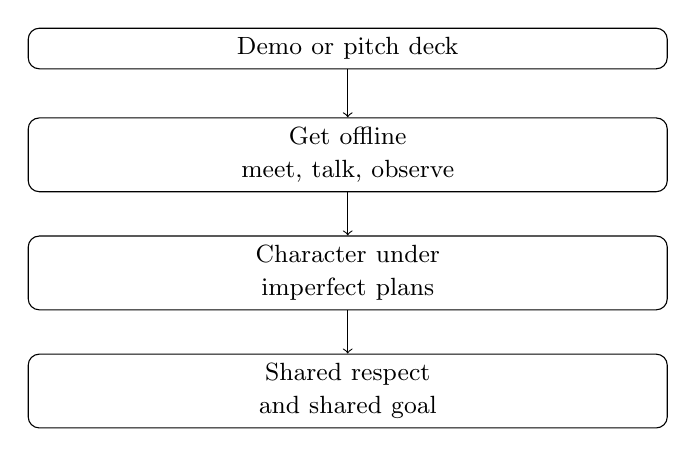
\begin{tikzpicture}[x=1cm,y=1cm]
\node[draw, rounded corners, text width=.65\linewidth, align=center] (a) at (0,0) {\small Demo or pitch deck};
\node[draw, rounded corners, text width=.65\linewidth, align=center] (b) at (0,-1.35) {\small Get offline\\\small meet, talk, observe};
\node[draw, rounded corners, text width=.65\linewidth, align=center] (c) at (0,-2.85) {\small Character under\\\small imperfect plans};
\node[draw, rounded corners, text width=.65\linewidth, align=center] (d) at (0,-4.35) {\small Shared respect\\\small and shared goal};
\draw[->] (a) -- (b);
\draw[->] (b) -- (c);
\draw[->] (c) -- (d);
\end{tikzpicture}
\end{figure}

The transcript around the later risk example is badly corrupted, so we should not rebuild the missing story in detail. The reliable endpoint is clear: different people have different risk profiles, and one has to be comfortable with one's own.

\section{Advice: Lift Others Up}

The closing question asks what Gen Z should know as it begins careers and aims at business leadership. Williams's answer ties back to the whole interview. Ask what you can do to help, not only what you can do to get ahead.

This is not separate from the earlier mechanics. It is the same operating principle at the level of a career. Help creates trust. Trust creates access. Access creates chances to learn, sell, invest, and lead. The person who only advances alone becomes, in Williams's warning, more alone.

The final rule is therefore relational rather than merely motivational:
\begin{equation}
\mathrm{Help}
\longrightarrow
\mathrm{Trust}
\longrightarrow
\mathrm{Opportunity}
\longrightarrow
\mathrm{Compounding\ career\ capital}.
\end{equation}

\section{Summary}

Williams's interview gives a compact commercial logic. Invest early, but do not confuse capital with focus. Coach the CEO toward the few things that matter. Sell by discovering the buyer's pain, not by performing a demo. Scale by preparing the next operating design before the doubling arrives. Treat career capital as skills plus relationships plus reputation. Keep enough life outside the office to sharpen the person inside the office. And when money is at risk, study character, because plans rarely unfold perfectly.